\chapter{KẾT QUẢ NGHIÊN CỨU}

\textbf{
\section{Đặc điểm màu răng theo bảng Vita 3D ở sinh viên trường Đại học Y Dược - Đại học Quốc Gia Hà Nội năm 2023.}}


%chèn ảnh giới tính vào đây
\begin{figure}[h]
    \centering
    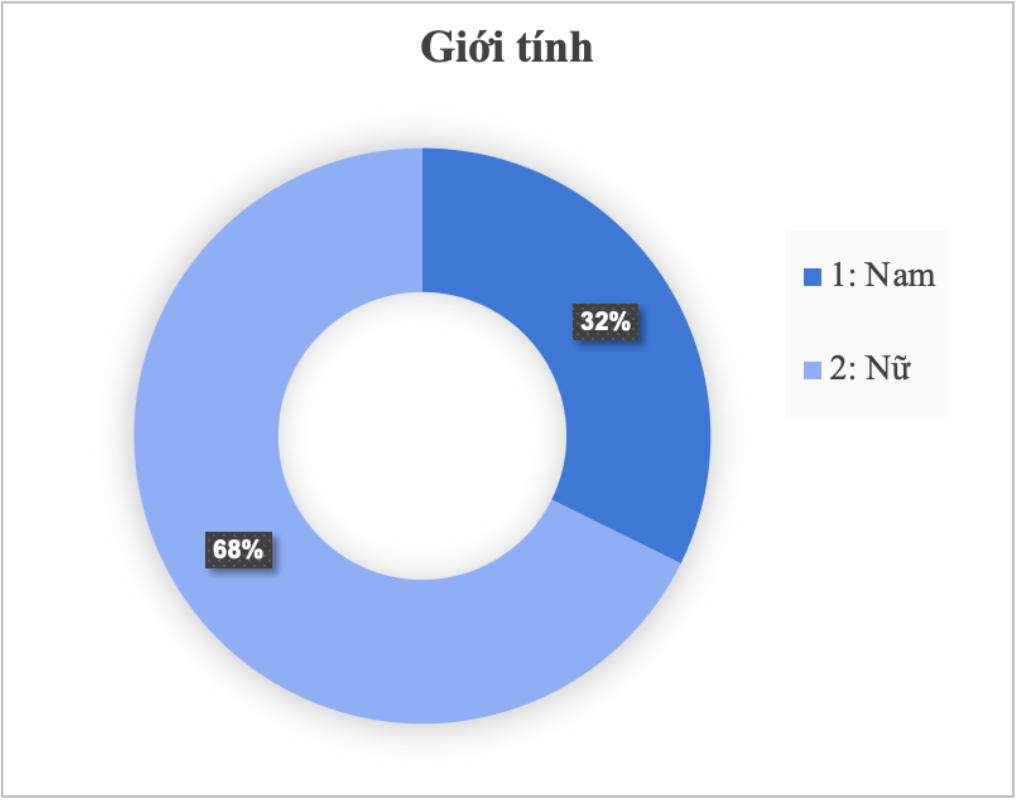
\includegraphics[width=0.8\columnwidth]{pictures/anh-gioi-tinh.jpeg}
    \caption{Biểu đồ tỷ lệ giới tính đối tượng nghiên cứu}
    \label{fig:yeu-to-chi-phoi-mau-sac-rang}
\end{figure}
\noindent
\textbf{Biểu đồ 3.1.1: Tỷ lệ nam nữ đối tượng nghiên cứu}

\noindent
\textbf{Nhận xét:}\par
\quad Tỷ lệ nữ cao gấp khoảng 2 lần so với nam.
\par

\noindent
\textbf{Bảng 3.1.1: Phân bố tiền sử người bệnh theo giới}
%chèn bảng vô đây
\begin{longtblr}[
caption=Phân bố tiền sử người bệnh theo giới
]{
  cells = {c},
  cell{1}{1} = {c=2,r=2}{},
  cell{1}{3} = {c=2}{},
  cell{1}{5} = {c=2}{},
  cell{1}{7} = {c=2}{},
  cell{3}{1} = {r=2}{},
  cell{5}{1} = {r=2}{},
  vlines,
  hline{1,3,5,7} = {-}{},
  hline{2} = {3-8}{},
  hline{4,6} = {2-8}{},
}
                                      &       & \textbf{Nam} &        & \textbf{Nữ} &        & \textbf{Tổng số} &        \\
                                      &       & n            & \%     & n           & \%     & n                & \%     \\
\textbf{Tiền sử sử dụng Tetracycline} & Không & 17           & 26,2\% & 34          & 52,3\% & 51               & 78,5\% \\
                                      & Có    & 4            & 6,2\%  & 10          & 15,4\% & 14               & 21,5\% \\
\textbf{Tiền sử chấn thương răng}     & Không & 20           & 30,8\% & 40          & 61,5\% & 60               & 92,3\% \\
                                      & Có    & 1            & 1,5\%  & 4           & 6,2\%  & 5                & 7,7\%  
\end{longtblr}
\vspace{1cm}
\noindent
\textbf{Nhận xét:}\par
\quad Tỷ lệ tiền sử sử dụng Tetracycline ở hai giới nam và nữ đều thấp (nữ: 21,5\% và nam: 6,2\%). Tỷ lệ có tiền sử chấn thương răng ở hai giới thấp (nữ: 7,7\% và nam: 1,5\%).\par

\noindent
\textbf{Bảng 3.1.2: Phân bố thói quen sử dụng đồ có màu của người bệnh theo giới}
%chèn bảng vô đây
\begin{longtblr}[
caption=Phân bố thói quen sử dụng đồ có màu của người bệnh theo giới
]{
  width = \linewidth,
  colspec = {Q[296]Q[92]Q[42]Q[106]Q[42]Q[106]Q[42]Q[106]Q[90]},
  row{even} = {c},
  row{3} = {c},
  row{5} = {c},
  row{7} = {c},
  row{9} = {c},
  row{11} = {c},
  cell{1}{1} = {c=2,r=2}{0.388\linewidth},
  cell{1}{3} = {c=2}{0.148\linewidth,c},
  cell{1}{5} = {c=2}{0.148\linewidth,c},
  cell{1}{7} = {c=2}{0.148\linewidth,c},
  cell{1}{9} = {r=2}{c},
  cell{3}{1} = {r=2}{},
  cell{3}{9} = {r=2}{},
  cell{5}{1} = {r=2}{},
  cell{5}{9} = {r=2}{},
  cell{7}{1} = {r=2}{},
  cell{7}{9} = {r=2}{},
  cell{9}{1} = {r=2}{},
  cell{9}{9} = {r=2}{},
  cell{11}{1} = {r=2}{},
  cell{11}{9} = {r=2}{},
  vlines,
  hline{1,3,5,7,9,11,13} = {-}{},
  hline{2} = {3-8}{},
  hline{4,6,8,10,12} = {2-8}{},
}
                           &       & \textbf{Nam} &         & \textbf{Nữ} &         & \textbf{Tổng số} &         & \textbf{P} \\
                           &       & n            & \%      & n           & \%      & n                & \%      &            \\
\textbf{Hút thuốc}         & Không & 15           & 23,10\% & 44          & 67,70\% & 59               & 90,80\% &  <0,01      \\
                           & Có    & 6            & 9,20\%  & 0           & 0,00\%  & 6                & 9,20\%  &            \\
\textbf{Cà phê}            & Không & 9            & 13,80\% & 26          & 40,00\% & 35               & 53,80\% &  >0,05      \\
                           & Có    & 12           & 18,50\% & 18          & 27,70\% & 30               & 46,20\% &            \\
\textbf{Nước chè}          & Không & 15           & 23,10\% & 38          & 58,50\% & 53               & 81,50\% &  >0,05      \\
                           & Có    & 6            & 9,20\%  & 6           & 9,20\%  & 12               & 18,50\% &            \\
\textbf{Coca Cola}         & Không & 5            & 7,70\%  & 21          & 32,30\% & 26               & 40,00\% &  >0,05      \\
                           & Có    & 16           & 24,60\% & 23          & 35,40\% & 39               & 60,00\% &            \\
\textbf{Nước uống sẫm màu} & Không & 6            & 9,20\%  & 30          & 46,20\% & 36               & 55,40\% &  <0,05      \\
                           & Có    & 15           & 23,10\% & 14          & 21,50\% & 29               & 44,60\% &            
\end{longtblr}
%đến đây là kết thúc bảng ạ

\noindent
\textbf{Nhận xét:}\par
\quad Thói quen sử dụng đồ có màu, cà phê, coca cola ở cả hai giới không có sự khác biệt nhiều (p>0,05). \par
\quad Thói quen sử dụng cocacola là cao nhất (60\%), uống cà phê chiếm 46,2\%, và đồ uống có màu khác chiếm khoảng 44,6\%. Hút thuốc lá chiếm 9,2\%. Hút thuốc lá chỉ gặp ở nam giới, không gặp ở nữ giới.


\noindent
\textbf{Bảng 3.1.3: Phân bố tình trạng vệ sinh răng miệng của người bệnh theo giới}\par

%chèn bảng vô đây
\begin{longtblr}[
caption=Phân bố tình trạng vệ sinh răng miệng của người bệnh theo giới
]{
  width = \linewidth,
  colspec = {Q[212]Q[302]Q[38]Q[79]Q[38]Q[79]Q[38]Q[79]Q[67]},
  row{2} = {c},
  column{2} = {c},
  column{9} = {c},
  cell{1}{1} = {c=2,r=2}{0.514\linewidth},
  cell{1}{3} = {c=2}{0.117\linewidth,c},
  cell{1}{5} = {c=2}{0.117\linewidth,c},
  cell{1}{7} = {c=2}{0.117\linewidth,c},
  cell{1}{9} = {r=2}{},
  cell{3}{1} = {r=3}{c},
  cell{3}{3} = {c},
  cell{3}{4} = {c},
  cell{3}{5} = {c},
  cell{3}{6} = {c},
  cell{3}{9} = {r=3}{},
  cell{4}{3} = {c},
  cell{4}{4} = {c},
  cell{4}{5} = {c},
  cell{4}{6} = {c},
  cell{5}{3} = {c},
  cell{5}{4} = {c},
  cell{5}{5} = {c},
  cell{5}{6} = {c},
  cell{6}{1} = {r=2}{c},
  cell{6}{3} = {c},
  cell{6}{4} = {c},
  cell{6}{5} = {c},
  cell{6}{6} = {c},
  cell{6}{9} = {r=2}{},
  cell{7}{3} = {c},
  cell{7}{4} = {c},
  cell{7}{5} = {c},
  cell{7}{6} = {c},
  cell{8}{1} = {r=4}{c},
  cell{8}{3} = {c},
  cell{8}{4} = {c},
  cell{8}{5} = {c},
  cell{8}{6} = {c},
  cell{8}{9} = {r=4}{},
  cell{9}{3} = {c},
  cell{9}{4} = {c},
  cell{9}{5} = {c},
  cell{9}{6} = {c},
  cell{10}{3} = {c},
  cell{10}{4} = {c},
  cell{10}{5} = {c},
  cell{10}{6} = {c},
  cell{11}{3} = {c},
  cell{11}{4} = {c},
  cell{11}{5} = {c},
  cell{11}{6} = {c},
  vlines,
  hline{1,3,6,8,12} = {-}{},
  hline{2} = {3-8}{},
  hline{4-5,7,9-11} = {2-8}{},
}
                              &                                  & \textbf{Nam} &        & \textbf{Nữ} &        & \textbf{Tổng số} &        & \textbf{P} \\
                              &                                  & n            & \%     & n           & \%     & n                & \%     &            \\
\textbf{Vệ sinh răng miệng}   & 1 lần/ngày                       & 0            & 0,0\%  & 0           & 0,0\%  & 0                & 0,0\%  & > 0,05       \\
                              & 2 lần/ngày                       & 17           & 26,2\% & 36          & 55,4\% & 53               & 81,5\% &            \\
                              & trên 2 lần/ngày                  & 4            & 6,2\%  & 8           & 12,3\% & 12               & 18,5\% &            \\
\textbf{Nước súc miệng}       & Không                           & 15           & 23,1\% & 32          & 49,2\% & 47               & 72,3\% & > 0,05       \\
                              & Có                               & 6            & 9,2\%  & 12          & 18,5\% & 18               & 27,7\% &            \\
\textbf{Lấy cao răng định kì} & Chưa bao giờ lấy cao răng        & 4            & 6,2\%  & 8           & 12,3\% & 12               & 18,5\% & > 0,05       \\
                              & Lấy cao răng 3 tháng 1 lần       & 0            & 0,0\%  & 4           & 6,2\%  & 4                & 6,2\%  &            \\
                              & Lấy cao 6 tháng 1 lần            & 12           & 18,5\% & 18          & 27,7\% & 30               & 46,2\% &            \\
                              & Trên 1 năm đi lấy cao răng 1 lần & 5            & 7,7\%  & 14          & 21,5\% & 19               & 29,2\% &            
\end{longtblr}

\noindent
\textbf{Nhận xét:}\par
\quad Tình trạng vệ sinh răng miệng ở hai giới tương đối đồng đều. \par
\quad Vệ sinh răng miệng 2 lần/ngày cao nhất, chiếm khoảng 81,5\%, không có ý nghĩa thống kê (p>0,05).\par
\quad Tỷ lệ sử dụng nước súc miệng có màu sẫm tương đối thấp, khoảng 27,7\%. \par
\quad Tình trạng chăm sóc răng miệng định kỳ 6 tháng 1 lần chiếm tỷ lệ khoảng 46,2\%. \par
\quad Tỷ lệ trên 1 năm đi lấy cao răng 1 lần chiếm khoảng 29,2\%. Chưa đi lấy cao răng bao giờ chiếm tỷ lệ 18,5\% và không có ý nghĩa thống kê (p>0,05).

\noindent
\textbf{Bảng 3.1.4: Phân bố đặc điểm của răng theo giới}\par

%chèn bảng vô đây
\begin{longtblr}[
caption=Phân bố đặc điểm của răng theo giới
]{
  width = \linewidth,
  colspec = {Q[202]Q[225]Q[42]Q[90]Q[42]Q[90]Q[42]Q[106]Q[83]},
  row{2} = {c},
  column{2} = {c},
  column{9} = {c},
  cell{1}{1} = {c=2,r=2}{0.427\linewidth},
  cell{1}{3} = {c=2}{0.132\linewidth,c},
  cell{1}{5} = {c=2}{0.132\linewidth,c},
  cell{1}{7} = {c=2}{0.148\linewidth,c},
  cell{1}{9} = {r=2}{},
  cell{3}{1} = {r=2}{c},
  cell{3}{3} = {c},
  cell{3}{4} = {c},
  cell{3}{5} = {c},
  cell{3}{6} = {c},
  cell{3}{9} = {r=2}{},
  cell{4}{3} = {c},
  cell{4}{4} = {c},
  cell{4}{5} = {c},
  cell{4}{6} = {c},
  cell{5}{1} = {r=2}{c},
  cell{5}{3} = {c},
  cell{5}{4} = {c},
  cell{5}{5} = {c},
  cell{5}{6} = {c},
  cell{5}{9} = {r=2}{},
  cell{6}{3} = {c},
  cell{6}{4} = {c},
  cell{6}{5} = {c},
  cell{6}{6} = {c},
  cell{7}{1} = {r=2}{c},
  cell{7}{3} = {c},
  cell{7}{4} = {c},
  cell{7}{5} = {c},
  cell{7}{6} = {c},
  cell{7}{9} = {r=2}{},
  cell{8}{3} = {c},
  cell{8}{4} = {c},
  cell{8}{5} = {c},
  cell{8}{6} = {c},
  cell{9}{1} = {r=2}{c},
  cell{9}{3} = {c},
  cell{9}{4} = {c},
  cell{9}{5} = {c},
  cell{9}{6} = {c},
  cell{9}{9} = {r=2}{},
  cell{10}{3} = {c},
  cell{10}{4} = {c},
  cell{10}{5} = {c},
  cell{10}{6} = {c},
  vlines,
  hline{1,3,5,7,9,11} = {-}{},
  hline{2} = {3-8}{},
  hline{4,6,8,10} = {2-8}{},
}
                       &                 & \textbf{Nam} &        & \textbf{Nữ} &        & \textbf{Tổng số} &         & \textbf{P} \\
                       &                 & n            & \%     & n           & \%     & n                & \%      &             \\
\textbf{Bề mặt răng}   & Nhẵn bóng       & 20           & 30,8\% & 40          & 61,5\% & 60               & 92,3\%  & >0,05        \\
                       & Sần sùi         & 1            & 1,5\%  & 4           & 6,2\%  & 5                & 7,7\%   &             \\
\textbf{Răng rạn nứt}  & Không           & 21           & 32,3\% & 43          & 66,2\% & 64               & 98,5\%  & >0,05        \\
                       & Có              & 0            & 0,0\%  & 1           & 1,5\%  & 1                & 1,5\%   &             \\
\textbf{Răng sâu}      & Không           & 21           & 32,3\% & 44          & 67,7\% & 65               & 100,0\% & 0           \\
                       & Có              & 0            & 0,0\%  & 0           & 0,0\%  & 0                & 0,0\%   &             \\
\textbf{Tính chất màu} & {Không đồng \\ nhất} & 1            & 1,5\%  & 7           & 10,8\% & 8                & 12,3\%  & >0,05        \\
                       & Đồng nhất       & 20           & 30,8\% & 37          & 56,9\% & 57               & 87,7\%  &             
\end{longtblr}

\noindent
\textbf{Nhận xét:}\par
\quad Tỷ lệ bề mặt răng nhẵn bóng (92,3\%) cao hơn so với bề mặt răng sần sùi (7,7\%), không có ý nghĩa thống kê (p>0,05). Đa số các răng không rạn nứt (98,5\%), không có ý nghĩa thống kê (p>0,05). Không có răng sâu nào. Tỷ lệ tính chất màu sắc răng đồng nhất là 87,7\%, cao hơn tỷ lệ tính chất màu sắc răng không đồng nhất khoảng 7 lần (12,3\%), không có ý nghĩa thống kê (p>0,05).\\
\noindent
\textbf{Bảng 3.1.5: Phân bố màu sắc giá trị màu (value) hàm trên theo nhóm răng}\par

\begin{longtblr}[
caption=Phân bố màu sắc giá trị màu (value) hàm trên theo nhóm răng
]{
  row{2} = {c},
  column{2} = {c},
  column{9} = {c},
  cell{1}{1} = {c=2,r=2}{},
  cell{1}{3} = {c=2}{c},
  cell{1}{5} = {c=2}{c},
  cell{1}{7} = {c=2}{c},
  cell{1}{9} = {r=2}{},
  cell{3}{1} = {r=5}{c},
  cell{3}{3} = {c},
  cell{3}{4} = {c},
  cell{3}{5} = {c},
  cell{3}{6} = {c},
  cell{3}{9} = {r=5}{},
  cell{4}{3} = {c},
  cell{4}{4} = {c},
  cell{4}{5} = {c},
  cell{4}{6} = {c},
  cell{5}{3} = {c},
  cell{5}{4} = {c},
  cell{5}{5} = {c},
  cell{5}{6} = {c},
  cell{6}{3} = {c},
  cell{6}{4} = {c},
  cell{6}{5} = {c},
  cell{6}{6} = {c},
  cell{7}{3} = {c},
  cell{7}{4} = {c},
  cell{7}{5} = {c},
  cell{7}{6} = {c},
  cell{8}{1} = {r=5}{c},
  cell{8}{3} = {c},
  cell{8}{4} = {c},
  cell{8}{5} = {c},
  cell{8}{6} = {c},
  cell{8}{9} = {r=5}{},
  cell{9}{3} = {c},
  cell{9}{4} = {c},
  cell{9}{5} = {c},
  cell{9}{6} = {c},
  cell{10}{3} = {c},
  cell{10}{4} = {c},
  cell{10}{5} = {c},
  cell{10}{6} = {c},
  cell{11}{3} = {c},
  cell{11}{4} = {c},
  cell{11}{5} = {c},
  cell{11}{6} = {c},
  cell{12}{3} = {c},
  cell{12}{4} = {c},
  cell{12}{5} = {c},
  cell{12}{6} = {c},
  cell{13}{1} = {r=5}{c},
  cell{13}{3} = {c},
  cell{13}{4} = {c},
  cell{13}{5} = {c},
  cell{13}{6} = {c},
  cell{13}{9} = {r=5}{},
  cell{14}{3} = {c},
  cell{14}{4} = {c},
  cell{14}{5} = {c},
  cell{14}{6} = {c},
  cell{15}{3} = {c},
  cell{15}{4} = {c},
  cell{15}{5} = {c},
  cell{15}{6} = {c},
  cell{16}{3} = {c},
  cell{16}{4} = {c},
  cell{16}{5} = {c},
  cell{16}{6} = {c},
  cell{17}{3} = {c},
  cell{17}{4} = {c},
  cell{17}{5} = {c},
  cell{17}{6} = {c},
  vlines,
  hline{1,3,8,13,18} = {-}{},
  hline{2} = {3-8}{},
  hline{4-7,9-12,14-17} = {2-8}{},
}
                                &        & \textbf{Nam} &        & \textbf{Nữ} &        & \textbf{Tổng số} &        & P    \\
                                &        & n            & \%     & n           & \%     & n                & \%     &      \\
\textbf{Nhóm răng cửa trên}     & Nhóm 1 & 0            & 0,0\%  & 1           & 1,5\%  & 1                & 1,5\%  & >0,05 \\
                                & Nhóm 2 & 9            & 13,8\% & 19          & 29,2\% & 28               & 43,1\% &      \\
                                & Nhóm 3 & 10           & 15,4\% & 23          & 35,4\% & 33               & 50,8\% &      \\
                                & Nhóm 4 & 2            & 3,1\%  & 1           & 1,5\%  & 3                & 4,6\%  &      \\
                                & Nhóm 5 & 0            & 0,0\%  & 0           & 0,0\%  & 0                & 0,0\%  &      \\
\textbf{Nhóm răng nanh trên}    & Nhóm 1 & 0            & 0,0\%  & 0           & 0,0\%  & 0                & 0,0\%  & >0,05 \\
                                & Nhóm 2 & 7            & 10,8\% & 19          & 29,2\% & 26               & 40,0\% &      \\
                                & Nhóm 3 & 11           & 16,9\% & 24          & 36,9\% & 35               & 53,8\% &      \\
                                & Nhóm 4 & 3            & 4,6\%  & 1           & 1,5\%  & 4                & 6,2\%  &      \\
                                & Nhóm 5 & 0            & 0,0\%  & 0           & 0,0\%  & 0                & 0,0\%  &      \\
\textbf{Nhóm răng hàm nhỏ trên} & Nhóm 1 & 0            & 0,0\%  & 1           & 1,5\%  & 1                & 1,5\%  & >0,05 \\
                                & Nhóm 2 & 8            & 12,3\% & 19          & 29,2\% & 27               & 41,5\% &      \\
                                & Nhóm 3 & 11           & 16,9\% & 24          & 36,9\% & 35               & 53,8\% &      \\
                                & Nhóm 4 & 2            & 3,1\%  & 0           & 0,0\%  & 2                & 3,1\%  &      \\
                                & Nhóm 5 & 0            & 0,0\%  & 0           & 0,0\%  & 0                & 0,0\%  &      
\end{longtblr}
%chèn bảng vô đây

\noindent
\textbf{Nhận xét:}\par
\quad Tỷ lệ phân bố màu sắc răng giá trị màu ở nhóm 3 là cao nhất ở cả 3 nhóm răng (nhóm răng cửa (50,8\%), nhóm răng nanh (53,8\%), nhóm răng hàm nhỏ (53,8\%)) và tương đối ngang nhau giữa hai giới nam và nữ (p>0,05).\par
\quad Tỷ lệ giá trị màu sắc răng ở nhóm 2 xếp sau với nhóm răng cửa khoảng 43\%, nhóm răng nanh khoảng 40\% và nhóm răng hàm nhỏ khoảng 41,5\%.\par
\quad Nhóm 1 chỉ chiếm tỷ lệ rất nhỏ là 1,5\% và không có đối tượng nào có màu sắc theo nhóm 5. Không có ý nghĩa thống kê (p>0,05).

\noindent
\textbf{Bảng 3.1.6: Phân bố màu sắc giá trị màu (value) hàm dưới theo nhóm răng
}\par
\begin{longtblr}[
caption=Phân bố màu sắc giá trị màu (value) hàm dưới theo nhóm răng
]{
  row{2} = {c},
  column{2} = {c},
  column{9} = {c},
  cell{1}{1} = {c=2,r=2}{},
  cell{1}{3} = {c=2}{c},
  cell{1}{5} = {c=2}{c},
  cell{1}{7} = {c=2}{c},
  cell{1}{9} = {r=2}{},
  cell{3}{1} = {r=5}{c},
  cell{3}{3} = {c},
  cell{3}{4} = {c},
  cell{3}{5} = {c},
  cell{3}{6} = {c},
  cell{3}{9} = {r=5}{},
  cell{4}{3} = {c},
  cell{4}{4} = {c},
  cell{4}{5} = {c},
  cell{4}{6} = {c},
  cell{5}{3} = {c},
  cell{5}{4} = {c},
  cell{5}{5} = {c},
  cell{5}{6} = {c},
  cell{6}{3} = {c},
  cell{6}{4} = {c},
  cell{6}{5} = {c},
  cell{6}{6} = {c},
  cell{7}{3} = {c},
  cell{7}{4} = {c},
  cell{7}{5} = {c},
  cell{7}{6} = {c},
  cell{8}{1} = {r=5}{c},
  cell{8}{3} = {c},
  cell{8}{4} = {c},
  cell{8}{5} = {c},
  cell{8}{6} = {c},
  cell{8}{9} = {r=5}{},
  cell{9}{3} = {c},
  cell{9}{4} = {c},
  cell{9}{5} = {c},
  cell{9}{6} = {c},
  cell{10}{3} = {c},
  cell{10}{4} = {c},
  cell{10}{5} = {c},
  cell{10}{6} = {c},
  cell{11}{3} = {c},
  cell{11}{4} = {c},
  cell{11}{5} = {c},
  cell{11}{6} = {c},
  cell{12}{3} = {c},
  cell{12}{4} = {c},
  cell{12}{5} = {c},
  cell{12}{6} = {c},
  cell{13}{1} = {r=5}{c},
  cell{13}{3} = {c},
  cell{13}{4} = {c},
  cell{13}{5} = {c},
  cell{13}{6} = {c},
  cell{13}{9} = {r=5}{},
  cell{14}{3} = {c},
  cell{14}{4} = {c},
  cell{14}{5} = {c},
  cell{14}{6} = {c},
  cell{15}{3} = {c},
  cell{15}{4} = {c},
  cell{15}{5} = {c},
  cell{15}{6} = {c},
  cell{16}{3} = {c},
  cell{16}{4} = {c},
  cell{16}{5} = {c},
  cell{16}{6} = {c},
  cell{17}{3} = {c},
  cell{17}{4} = {c},
  cell{17}{5} = {c},
  cell{17}{6} = {c},
  vlines,
  hline{1,3,8,13,18} = {-}{},
  hline{2} = {3-8}{},
  hline{4-7,9-12,14-17} = {2-8}{},
}
                                &        & \textbf{Nam} &        & \textbf{Nữ} &        & \textbf{Tổng số} &        & \textbf{P} \\
                                &        & n            & \%     & n           & \%     & n                & \%     &            \\
\textbf{Nhóm răng cửa dưới}     & Nhóm 1 & 0            & 0,0\%  & 0           & 0,0\%  & 0                & 0,0\%  & <0,05       \\
                                & Nhóm 2 & 6            & 9,4\%  & 11          & 17,2\% & 17               & 26,6\% &            \\
                                & Nhóm 3 & 12           & 18,8\% & 32          & 50,0\% & 44               & 68,8\% &            \\
                                & Nhóm 4 & 3            & 4,7\%  & 0           & 0,0\%  & 3                & 4,7\%  &            \\
                                & Nhóm 5 & 0            & 0,0\%  & 0           & 0,0\%  & 0                & 0,0\%  &            \\
\textbf{Nhóm răng nanh dưới}    & Nhóm 1 & 0            & 0,0\%  & 0           & 0,0\%  & 0                & 0,0\%  & >0,05       \\
                                & Nhóm 2 & 5            & 7,8\%  & 11          & 17,2\% & 16               & 25,0\% &            \\
                                & Nhóm 3 & 11           & 17,2\% & 28          & 43,8\% & 39               & 60,9\% &            \\
                                & Nhóm 4 & 5            & 7,8\%  & 4           & 6,3\%  & 9                & 14,1\% &            \\
                                & Nhóm 5 & 0            & 0,0\%  & 0           & 0,0\%  & 0                & 0,0\%  &            \\
\textbf{Nhóm răng hàm nhỏ dưới} & Nhóm 1 & 0            & 0,0\%  & 0           & 0,0\%  & 0                & 0,0\%  & <0,05       \\
                                & Nhóm 2 & 5            & 7,8\%  & 11          & 17,2\% & 16               & 25,0\% &            \\
                                & Nhóm 3 & 13           & 20,3\% & 32          & 50,0\% & 45               & 70,3\% &            \\
                                & Nhóm 4 & 3            & 4,7\%  & 0           & 0,0\%  & 3                & 4,7\%  &            \\
                                & Nhóm 5 & 0            & 0,0\%  & 0           & 0,0\%  & 0                & 0,0\%  &            
\end{longtblr}
%chèn bảng vô đây

\noindent
\textbf{Nhận xét:}\par
\quad Tỷ lệ phân bố giá trị màu sắc răng ở nhóm 3 là cao nhất ở cả 3 nhóm răng (nhóm răng cửa (68,8\%), nhóm răng nanh (6\%), nhóm răng hàm nhỏ(70,3\%)) và tương đối ngang nhau giữa hai giới nam và nữ. \par
\quad Tỷ lệ giá trị màu sắc răng ở nhóm 2 xếp sau với nhóm răng cửa khoảng 26,6\%, nhóm răng nanh khoảng 25\% và nhóm răng hàm nhỏ khoảng 25\%. Nhóm 1 và nhóm 5 không có đối tượng nào.\par
\quad Tỷ lệ phân bố màu sắc răng ở nhóm răng cửa dưới và nhóm răng hàm nhỏ dưới là có ý nghĩa thống kê (p<0,05) còn ở nhóm răng nanh dưới không có ý nghĩa thống kê (p>0,05).

\noindent
\textbf{Bảng 3.1.7: Phân bố màu sắc răng theo độ bão hoà và nhóm răng}\par

%chèn bảng vô đây
\begin{longtblr}[
caption=Phân bố màu sắc răng theo độ bão hoà và nhóm răng
]{
  row{2} = {c},
  column{2} = {c},
  column{9} = {c},
  cell{1}{1} = {c=2,r=2}{},
  cell{1}{3} = {c=2}{c},
  cell{1}{5} = {c=2}{c},
  cell{1}{7} = {c=2}{c},
  cell{1}{9} = {r=2}{},
  cell{3}{1} = {r=3}{c},
  cell{3}{3} = {c},
  cell{3}{4} = {c},
  cell{3}{5} = {c},
  cell{3}{6} = {c},
  cell{3}{9} = {r=3}{},
  cell{4}{3} = {c},
  cell{4}{4} = {c},
  cell{4}{5} = {c},
  cell{4}{6} = {c},
  cell{5}{3} = {c},
  cell{5}{4} = {c},
  cell{5}{5} = {c},
  cell{5}{6} = {c},
  cell{6}{1} = {r=3}{c},
  cell{6}{3} = {c},
  cell{6}{4} = {c},
  cell{6}{5} = {c},
  cell{6}{6} = {c},
  cell{6}{9} = {r=3}{},
  cell{7}{3} = {c},
  cell{7}{4} = {c},
  cell{7}{5} = {c},
  cell{7}{6} = {c},
  cell{8}{3} = {c},
  cell{8}{4} = {c},
  cell{8}{5} = {c},
  cell{8}{6} = {c},
  cell{9}{1} = {r=3}{c},
  cell{9}{3} = {c},
  cell{9}{4} = {c},
  cell{9}{5} = {c},
  cell{9}{6} = {c},
  cell{9}{9} = {r=3}{},
  cell{10}{3} = {c},
  cell{10}{4} = {c},
  cell{10}{5} = {c},
  cell{10}{6} = {c},
  cell{11}{3} = {c},
  cell{11}{4} = {c},
  cell{11}{5} = {c},
  cell{11}{6} = {c},
  cell{12}{1} = {r=3}{c},
  cell{12}{3} = {c},
  cell{12}{4} = {c},
  cell{12}{5} = {c},
  cell{12}{6} = {c},
  cell{12}{9} = {r=3}{},
  cell{13}{3} = {c},
  cell{13}{4} = {c},
  cell{13}{5} = {c},
  cell{13}{6} = {c},
  cell{14}{3} = {c},
  cell{14}{4} = {c},
  cell{14}{5} = {c},
  cell{14}{6} = {c},
  cell{15}{1} = {r=3}{c},
  cell{15}{3} = {c},
  cell{15}{4} = {c},
  cell{15}{5} = {c},
  cell{15}{6} = {c},
  cell{15}{9} = {r=3}{},
  cell{16}{3} = {c},
  cell{16}{4} = {c},
  cell{16}{5} = {c},
  cell{16}{6} = {c},
  cell{17}{3} = {c},
  cell{17}{4} = {c},
  cell{17}{5} = {c},
  cell{17}{6} = {c},
  cell{18}{1} = {r=3}{c},
  cell{18}{3} = {c},
  cell{18}{4} = {c},
  cell{18}{5} = {c},
  cell{18}{6} = {c},
  cell{18}{9} = {r=3}{},
  cell{19}{3} = {c},
  cell{19}{4} = {c},
  cell{19}{5} = {c},
  cell{19}{6} = {c},
  cell{20}{3} = {c},
  cell{20}{4} = {c},
  cell{20}{5} = {c},
  cell{20}{6} = {c},
  vlines,
  hline{1,3,6,9,12,15,18,21} = {-}{},
  hline{2} = {3-8}{},
  hline{4-5,7-8,10-11,13-14,16-17,19-20} = {2-8}{},
}
                                &   & \textbf{Nam} &        & \textbf{Nữ} &        & \textbf{Tổng số} &        & P    \\
                                &   & n             & \%     & n           & \%     & n                & \%     &      \\
\textbf{Nhóm răng cửa trên}     & L & 2             & 3,1\%  & 2           & 3,1\%  & 4                & 6,2\%  & >0,05 \\
                                & M & 13            & 20,0\% & 21          & 32,3\% & 34               & 52,3\% &      \\
                                & R & 6             & 9,2\%  & 21          & 32,3\% & 27               & 41,5\% &      \\
\textbf{Nhóm răng nanh trên}    & L & 3             & 4,6\%  & 6           & 9,2\%  & 9                & 13,8\% & >0,05 \\
                                & M & 13            & 20,0\% & 30          & 46,2\% & 43               & 66,2\% &      \\
                                & R & 5             & 7,7\%  & 8           & 12,3\% & 13               & 20,0\% &      \\
\textbf{Nhóm răng hàm nhỏ trên} & L & 4             & 6,2\%  & 3           & 4,6\%  & 7                & 10,8\% & >0,05 \\
                                & M & 10            & 15,4\% & 22          & 33,8\% & 32               & 49,2\% &      \\
                                & R & 7             & 10,8\% & 19          & 29,2\% & 26               & 40,0\% &      \\
\textbf{Nhóm răng cửa dưới}     & L & 3             & 4,7\%  & 4           & 6,3\%  & 7                & 10,9\% & >0,05 \\
                                & M & 13            & 20,3\% & 29          & 45,3\% & 42               & 65,6\% &      \\
                                & R & 5             & 7,8\%  & 10          & 15,6\% & 15               & 23,4\% &      \\
\textbf{Nhóm răng nanh dưới}    & L & 2             & 3,1\%  & 8           & 12,5\% & 10               & 15,6\% & >0,05 \\
                                & M & 17            & 26,6\% & 27          & 42,2\% & 44               & 68,8\% &      \\
                                & R & 2             & 3,1\%  & 8           & 12,5\% & 10               & 15,6\% &      \\
\textbf{Nhóm răng hàm nhỏ dưới} & L & 2             & 3,1\%  & 3           & 4,7\%  & 5                & 7,8\%  & >0,05 \\
                                & M & 10            & 15,6\% & 21          & 32,8\% & 31               & 48,4\% &      \\
                                & R & 9             & 14,1\% & 19          & 29,7\% & 28               & 43,8\% &      
\end{longtblr}

\noindent
\textbf{Nhận xét:}\par
\quad Tỷ lệ các răng ở đối tượng nghiên có màu trung tính chiếm phần lớn ở cả hai giới nam và nữ (>46\%). \par
\quad Tỷ lệ màu đỏ thấp hơn còn tỷ lệ màu vàng là thấp nhất ở cả nam và nữ và không có ý nghĩa thống kê (p>0,05).

\textbf{
\section{Xác định nhu cầu điều trị ở nhóm đối tượng trên}}

\noindent
\textbf{Bảng 3.2.1: Phân bố mức độ sự đổi màu theo giới}\par

%chèn bảng vô đây
\begin{longtblr}[
caption=Phân bố mức độ sự đổi màu theo giới
]{
  cells = {c},
  cell{1}{1} = {r=2}{},
  cell{1}{2} = {c=2}{},
  cell{1}{4} = {c=2}{},
  cell{1}{6} = {c=2}{},
  cell{1}{8} = {r=2}{},
  cell{3}{8} = {r=4}{},
  vlines,
  hline{1,3,7} = {-}{},
  hline{2} = {2-7}{},
  hline{4-6} = {1-7}{},
}
                                    & \textbf{Nam} &        & \textbf{Nữ} &        & \textbf{Tổng số} &        & \textbf{P} \\
                                    & n            & \%     & n           & \%     & n                & \%     &            \\
\textbf{Đổi màu nghiêm trọng}       & 2            & 3,1\%  & 1           & 1,5\%  & 3                & 4,6\%  & >0,05       \\
\textbf{Đổi màu vừa phải}           & 19           & 29,2\% & 40          & 61,5\% & 59               & 90,8\% &            \\
\textbf{Đổi màu nhẹ}                & 0            & 0,0\%  & 3           & 4,6\%  & 3                & 4,6\%  &            \\
\textbf{Đổi màu nhẹ hoặc đốm trắng} & 0            & 0,0\%  & 0           & 0,0\%  & 0                & 0,0\%  &            
\end{longtblr}

\noindent
\textbf{Nhận xét:}\par
\quad Sự đổi màu răng ở các đối tượng nghiên cứu là như nhau ở hai giới nam và nữ (p>0,05). \par
\quad Tỷ lệ đổi màu vừa phải cao nhất (90,7\%), tỷ lệ đổi màu nghiêm trọng thấp hơn (4,6\%).

\noindent
\textbf{Bảng 3.2.2: Phân bố vị trí đổi màu răng theo giới}\par

\begin{longtblr}[
  label = none,
  entry = none,
]{
  row{2} = {c},
  column{8} = {c},
  cell{1}{1} = {r=2}{},
  cell{1}{2} = {c=2}{c},
  cell{1}{4} = {c=2}{c},
  cell{1}{6} = {c=2}{c},
  cell{1}{8} = {r=2}{},
  cell{3}{1} = {c},
  cell{3}{2} = {c},
  cell{3}{3} = {c},
  cell{3}{4} = {c},
  cell{3}{5} = {c},
  cell{3}{8} = {r=5}{},
  cell{4}{1} = {c},
  cell{4}{2} = {c},
  cell{4}{3} = {c},
  cell{4}{4} = {c},
  cell{4}{5} = {c},
  cell{5}{1} = {c},
  cell{5}{2} = {c},
  cell{5}{3} = {c},
  cell{5}{4} = {c},
  cell{5}{5} = {c},
  cell{6}{1} = {c},
  cell{6}{2} = {c},
  cell{6}{3} = {c},
  cell{6}{4} = {c},
  cell{6}{5} = {c},
  cell{7}{1} = {c},
  cell{7}{2} = {c},
  cell{7}{3} = {c},
  cell{7}{4} = {c},
  cell{7}{5} = {c},
  vlines,
  hline{1,3,8} = {-}{},
  hline{2} = {2-7}{},
  hline{4-7} = {1-7}{},
}
                                                         & \textbf{Nam} &        & \textbf{Nữ} &        & \textbf{Tổng số} &        & \textbf{P} \\
                                                         & n            & \%     & n           & \%     & n                & \%     &            \\
{\textbf{Phân bố nhiều vết}\\\textbf{đậm nhạt đồng đều}} & 1            & 1,5\%  & 1           & 1,5\%  & 2                & 3,1\%  & >0,05       \\
\textbf{Phân bố đều các răng}                            & 10           & 15,4\% & 16          & 24,6\% & 26               & 40,0\% &            \\
{\textbf{Phân bố trên các}\\\textbf{răng phía trước}}    & 0            & 0,0\%  & 1           & 1,5\%  & 1                & 1,5\%  &            \\
{\textbf{Phân bố ngẫu nhiên}\\\textbf{trên răng}}        & 0            & 0,0\%  & 2           & 3,1\%  & 2                & 3,1\%  &            \\
{\textbf{Phân bố ở ít răng}\\\textbf{hoặc một răng}}     & 10           & 15,4\% & 24          & 36,9\% & 34               & 52,3\% &            
\end{longtblr}
%chèn bảng vô đây


\noindent
\textbf{Nhận xét:}\par
\quad Tỷ lệ phân bố vị trí đổi màu răng ở hai giới cũng có sự tương đồng (p>0,05). \par
\quad Phân bố ở ít răng hoặc một răng chiếm tỷ lệ cao nhất (52,3\%). Tỷ lệ phân bố đều ở các răng thấp hơn (40\%). \par
\quad Tỷ lệ phân bố nhiều vết đậm nhạt đồng đều là 3\%. \par
\quad Tỷ lệ phân bố trên các răng phía trước thấp nhất, chiếm 1,5\%.

\noindent
\textbf{Bảng 3.2.3: Phân bố ảnh hưởng của màu sắc răng tới người bệnh theo giới}\par

%chèn bảng vô đây
\begin{longtblr}[
caption=Phân bố ảnh hưởng của màu sắc răng tới người bệnh theo giới
]{
  width = \linewidth,
  colspec = {Q[402]Q[31]Q[100]Q[48]Q[100]Q[48]Q[100]Q[92]},
  row{2} = {c},
  column{8} = {c},
  cell{1}{1} = {r=2}{},
  cell{1}{2} = {c=2}{0.131\linewidth,c},
  cell{1}{4} = {c=2}{0.148\linewidth,c},
  cell{1}{6} = {c=2}{0.148\linewidth,c},
  cell{1}{8} = {r=2}{},
  cell{3}{1} = {c},
  cell{3}{2} = {c},
  cell{3}{3} = {c},
  cell{3}{4} = {c},
  cell{3}{5} = {c},
  cell{3}{8} = {r=5}{},
  cell{4}{1} = {c},
  cell{4}{2} = {c},
  cell{4}{3} = {c},
  cell{4}{4} = {c},
  cell{4}{5} = {c},
  cell{5}{1} = {c},
  cell{5}{2} = {c},
  cell{5}{3} = {c},
  cell{5}{4} = {c},
  cell{5}{5} = {c},
  cell{6}{1} = {c},
  cell{6}{2} = {c},
  cell{6}{3} = {c},
  cell{6}{4} = {c},
  cell{6}{5} = {c},
  cell{7}{1} = {c},
  cell{7}{2} = {c},
  cell{7}{3} = {c},
  cell{7}{4} = {c},
  cell{7}{5} = {c},
  vlines,
  hline{1,3,8} = {-}{},
  hline{2} = {2-7}{},
  hline{4-7} = {1-7}{},
}
                                     & \textbf{Nam} &        & \textbf{Nữ} &        & \textbf{Tổng số} &        & \textbf{P} \\
                                     & n            & \%     & n           & \%     & n                & \%     &             \\
\textbf{Rất mất tự tin}              & 1            & 1,5\%  & 0           & 0,0\%  & 1                & 1,5\%  & >0,05        \\
\textbf{Mất tự tin}                  & 1            & 1,5\%  & 1           & 1,5\%  & 2                & 3,1\%  &             \\
\textbf{Mất tự tin một chút}         & 9            & 13,8\% & 31          & 47,7\% & 40               & 61,5\% &             \\
\textbf{Không mất tự tin chút nào}   & 8            & 12,3\% & 12          & 18,5\% & 20               & 30,8\% &             \\
\textbf{Hoàn toàn tự tin là rất đẹp} & 2            & 3,1\%  & 0           & 0,0\%  & 2                & 3,1\%  &             
\end{longtblr}

\noindent
\textbf{Nhận xét:}\par
\quad Tỷ lệ của ảnh hưởng màu sắc răng tới người bệnh khiến người bệnh mất tự tin một chút là cao nhất, chiếm khoảng 61,5\%.\par
\quad Tỷ lệ người bệnh không mất tự tin chút nào thấp hơn, khoảng 30,8\%. \par
\quad Tỷ lệ người bệnh hoàn toàn tự tin là rất đẹp và mất tự tin là ngang nhau, khoảng 3\%. \par
\quad Tỷ lệ này không có ý nghĩa thống kê (p>0,05).

\noindent
\textbf{Bảng 3.2.4: Phân bố nhu cầu làm trắng theo giới}\par

%chèn bảng vô đây
\begin{longtblr}[
caption=Phân bố nhu cầu làm trắng theo giới
]{
  width = \linewidth,
  colspec = {Q[235]Q[60]Q[127]Q[60]Q[127]Q[60]Q[127]Q[113]},
  row{2} = {c},
  column{8} = {c},
  cell{1}{1} = {r=2}{},
  cell{1}{2} = {c=2}{0.187\linewidth,c},
  cell{1}{4} = {c=2}{0.187\linewidth,c},
  cell{1}{6} = {c=2}{0.187\linewidth,c},
  cell{1}{8} = {r=2}{},
  cell{3}{1} = {c},
  cell{3}{2} = {c},
  cell{3}{3} = {c},
  cell{3}{4} = {c},
  cell{3}{5} = {c},
  cell{3}{8} = {r=5}{},
  cell{4}{1} = {c},
  cell{4}{2} = {c},
  cell{4}{3} = {c},
  cell{4}{4} = {c},
  cell{4}{5} = {c},
  cell{5}{1} = {c},
  cell{5}{2} = {c},
  cell{5}{3} = {c},
  cell{5}{4} = {c},
  cell{5}{5} = {c},
  cell{6}{1} = {c},
  cell{6}{2} = {c},
  cell{6}{3} = {c},
  cell{6}{4} = {c},
  cell{6}{5} = {c},
  cell{7}{1} = {c},
  cell{7}{2} = {c},
  cell{7}{3} = {c},
  cell{7}{4} = {c},
  cell{7}{5} = {c},
  vlines,
  hline{1,3,8} = {-}{},
  hline{2} = {2-7}{},
  hline{4-7} = {1-7}{},
}
                    & \textbf{Nam} &        & \textbf{Nữ} &        & \textbf{Tổng số} &        & \textbf{P} \\
                    & n            & \%     & n           & \%     & n                & \%     &            \\
\textbf{Cao}        & 1            & 1,5\%  & 1           & 1,5\%  & 2                & 3,1\%  & >0,05       \\
\textbf{Trung bình} & 12           & 18,5\% & 31          & 47,7\% & 43               & 66,2\% &            \\
\textbf{Mong muốn}  & 5            & 7,7\%  & 7           & 10,8\% & 12               & 18,5\% &            \\
\textbf{Khuyến cáo} & 2            & 3,1\%  & 3           & 4,6\%  & 5                & 7,7\%  &            \\
\textbf{Có thể}     & 1            & 1,5\%  & 2           & 3,1\%  & 3                & 4,6\%  &            
\end{longtblr}

\noindent
\textbf{Nhận xét:}\par
\quad Tỷ lệ nhu cầu làm trắng răng mức trung bình là cao nhất ở cả hai giới nam và nữ, chiếm khoảng 66,2\%. \par
\quad Tỷ lệ nhu cầu làm trắng răng mức mong muốn thấp hơn, chiếm 18,5\%. \par
\quad Tỷ lệ nhu cầu làm trắng răng mức khuyến cáo là 7,7\%, mức có thể là 4,6\% và ở mức cao là 3\%. Tỷ lệ này không có ý nghĩa thống kê (p>0,05).

\noindent
\textbf{Bảng 3.2.5: Phân bố mong muốn làm trắng răng của người bệnh theo giới}\par

%chèn bảng vô đây
\begin{longtblr}[
caption=Phân bố mong muốn làm trắng răng của người bệnh theo giới
]{
  width = \linewidth,
  colspec = {Q[448]Q[29]Q[92]Q[44]Q[92]Q[44]Q[92]Q[85]},
  row{2} = {c},
  column{8} = {c},
  cell{1}{1} = {r=2}{},
  cell{1}{2} = {c=2}{0.121\linewidth,c},
  cell{1}{4} = {c=2}{0.136\linewidth,c},
  cell{1}{6} = {c=2}{0.136\linewidth,c},
  cell{1}{8} = {r=2}{},
  cell{3}{1} = {c},
  cell{3}{2} = {c},
  cell{3}{3} = {c},
  cell{3}{4} = {c},
  cell{3}{5} = {c},
  cell{3}{8} = {r=5}{},
  cell{4}{1} = {c},
  cell{4}{2} = {c},
  cell{4}{3} = {c},
  cell{4}{4} = {c},
  cell{4}{5} = {c},
  cell{5}{1} = {c},
  cell{5}{2} = {c},
  cell{5}{3} = {c},
  cell{5}{4} = {c},
  cell{5}{5} = {c},
  cell{6}{1} = {c},
  cell{6}{2} = {c},
  cell{6}{3} = {c},
  cell{6}{4} = {c},
  cell{6}{5} = {c},
  cell{7}{1} = {c},
  cell{7}{2} = {c},
  cell{7}{3} = {c},
  cell{7}{4} = {c},
  cell{7}{5} = {c},
  vlines,
  hline{1,3,8} = {-}{},
  hline{2} = {2-7}{},
  hline{4-7} = {1-7}{},
}
                                                                                                   & \textbf{Nam} &        & \textbf{Nữ} &        & \textbf{Tổng số} &        & \textbf{P} \\
                                                                                                   & n            & \%     & n           & \%     & n                & \%     &            \\
\textbf{Rất muốn được trắng hơn}                                                                   & 0            & 0,0\%  & 2           & 3,1\%  & 2                & 3,1\%  & >0,05       \\
\textbf{Muốn răng được trắng hơn}                                                                  & 9            & 13,8\% & 26          & 40,0\% & 35               & 53,8\% &            \\
{\textbf{Thấy răng có nhiễm màu}\\\textbf{ và muốn các răng đó}\\\textbf{ sáng hơn}}                           & {\\4}            & {\\6,2\%}  & {\\3 }          & {\\4,6\% } & {\\7 }               & {\\10,8\%} &            \\
{\textbf{Nếu những răng nhiễm}\\\textbf{ màu sáng hơn thì tốt}}                                     &{\centering 4 }             & 6,2\%  & 4           & 6,2\%  & 8                & 12,3\% &            \\
{\textbf{Thấy có răng nhiễm màu}\\\textbf{ nhưng không quan tâm,}\\\textbf{ đợi làm trắng răng sau}} & {\\4}            & {\\6,2\% } & {\\9}           &{\\ 13,8\%}& {\\13 }              & {\\20,0\%} &            
\end{longtblr}

\noindent
\textbf{Nhận xét:}\par
\quad Tỷ lệ muốn răng được trắng hơn ở cả nam và nữ đều cao nhất (53,8\%), đặc biệt là nữ (74,3\% trong tổng nữ). Tỷ lệ đối tượng hiện tại đang không quan tâm và đợi làm trắng sau thấp hơn (khoảng 20\%). \par
\quad Tỷ lệ rất muốn được trắng hơn là thấp nhất, chỉ có 3,1\% và đều ở nữ giới và không có ý nghĩa thống kê (p>0,05).

\noindent
\textbf{Bảng 3.2.6: Phân bố màu sắc nhu cầu làm trắng theo mong muốn của người bệnh}\par

%chèn bảng vô đây
\begin{longtblr}[
caption=Phân bố màu sắc nhu cầu làm trắng theo mong muốn của người bệnh
]{
  row{2} = {c},
  cell{1}{1} = {r=2}{},
  cell{1}{2} = {c=2}{c},
  cell{1}{4} = {c=2}{c},
  cell{1}{6} = {c=2}{c},
  cell{1}{8} = {r=2}{c},
  cell{3}{1} = {c},
  cell{3}{2} = {c},
  cell{3}{3} = {c},
  cell{3}{4} = {c},
  cell{3}{5} = {c},
  cell{3}{8} = {r=4}{},
  cell{4}{1} = {c},
  cell{4}{2} = {c},
  cell{4}{3} = {c},
  cell{4}{4} = {c},
  cell{4}{5} = {c},
  cell{5}{1} = {c},
  cell{5}{2} = {c},
  cell{5}{3} = {c},
  cell{5}{4} = {c},
  cell{5}{5} = {c},
  cell{6}{1} = {c},
  cell{6}{2} = {c},
  cell{6}{3} = {c},
  cell{6}{4} = {c},
  cell{6}{5} = {c},
  cell{7}{1} = {c},
  cell{7}{2} = {c},
  cell{7}{3} = {c},
  cell{7}{4} = {c},
  cell{7}{5} = {c},
  cell{7}{8} = {c},
  cell{8}{1} = {c},
  cell{8}{2} = {c},
  cell{8}{3} = {c},
  cell{8}{4} = {c},
  cell{8}{5} = {c},
  cell{8}{8} = {r=4}{},
  cell{9}{1} = {c},
  cell{9}{2} = {c},
  cell{9}{3} = {c},
  cell{9}{4} = {c},
  cell{9}{5} = {c},
  cell{10}{1} = {c},
  cell{10}{2} = {c},
  cell{10}{3} = {c},
  cell{10}{4} = {c},
  cell{10}{5} = {c},
  cell{11}{1} = {c},
  cell{11}{2} = {c},
  cell{11}{3} = {c},
  cell{11}{4} = {c},
  cell{11}{5} = {c},
  vlines,
  hline{1,3,12} = {-}{},
  hline{2} = {2-7}{},
  hline{4-11} = {1-7}{},
}
                  & \textbf{Nam} &       & \textbf{Nữ} &        & \textbf{Tổng số} &        & \textbf{P} \\
                  & n            & \%    & n           & \%     & n                & \%     &            \\
\textbf{Màu khác} & 2            & 3,1\% & 4           & 6,2\%  & 6                & 9,2\%  &            \\
\textbf{2M3}      & 1            & 1,5\% & 0           & 0,0\%  & 1                & 1,5\%  &            \\
\textbf{2M2}      & 1            & 1,5\% & 0           & 0,0\%  & 1                & 1,5\%  &            \\
\textbf{2M1}      & 5            & 7,7\% & 5           & 7,7\%  & 10               & 15,4\% &            \\
\textbf{1M2}      & 5            & 7,7\% & 6           & 9,2\%  & 11               & 16,9\% & >0,05       \\
\textbf{1M1}      & 3            & 4,6\% & 16          & 24,6\% & 19               & 29,2\% &            \\
\textbf{0M3}      & 0            & 0,0\% & 6           & 9,2\%  & 6                & 9,2\%  &            \\
\textbf{0M2}      & 2            & 3,1\% & 5           & 7,7\%  & 7                & 10,8\% &            \\
\textbf{0M1}      & 2            & 3,1\% & 2           & 3,1\%  & 4                & 6,2\%  &            
\end{longtblr}

\noindent
\textbf{Nhận xét:}\par
\quad Tỷ lệ màu sắc mong muốn của người bệnh ở màu 1M1 ở nữ là cao nhất, chiếm 36,4\% tổng số.\par
\quad Tỷ lệ màu sắc mong muốn của nữ giới ở màu 0M3 và 1M2 là như nhau (13,6\%). \par
\quad Tỷ lệ màu sắc mong muốn của nam giới ở màu 2M1 và 1M2 là cao nhất (7.7\%). \par
\quad Tỷ lệ màu sắc mong muốn ở nhóm 0 ở nữ giới cao hơn nam giới (ở nữ: 29,5\%; ở nam: 19\%). Tỷ lệ này không có ý nghĩa thống kê (p>0,05).

\noindent
\textbf{Bảng 3.2.7: Phân bố nhu cầu làm trắng răng theo mong muốn người bệnh và theo sinh viên các năm}\par
%chèn bảng vô đây
\begin{longtblr}[
caption=Phân bố nhu cầu làm trắng răng theo mong muốn người bệnh và theo sinh viên các năm
]{
  width = \linewidth,
  colspec = {Q[233]Q[29]Q[65]Q[35]Q[69]Q[35]Q[69]Q[31]Q[71]Q[27]Q[69]Q[35]Q[69]Q[58]},
  row{2} = {c},
  cell{1}{1} = {r=2}{},
  cell{1}{2} = {c=2}{0.094\linewidth,c},
  cell{1}{4} = {c=2}{0.104\linewidth,c},
  cell{1}{6} = {c=2}{0.104\linewidth,c},
  cell{1}{8} = {c=2}{0.102\linewidth,c},
  cell{1}{10} = {c=2}{0.096\linewidth,c},
  cell{1}{12} = {c=2}{0.104\linewidth,c},
  cell{1}{14} = {r=2}{c},
  cell{3}{1} = {c},
  cell{3}{2} = {c},
  cell{3}{3} = {c},
  cell{3}{4} = {c},
  cell{3}{5} = {c},
  cell{3}{6} = {c},
  cell{3}{7} = {c},
  cell{3}{8} = {c},
  cell{3}{9} = {c},
  cell{3}{10} = {c},
  cell{3}{11} = {c},
  cell{3}{13} = {c},
  cell{3}{14} = {r=2}{},
  cell{4}{1} = {c},
  cell{4}{2} = {c},
  cell{4}{3} = {c},
  cell{4}{4} = {c},
  cell{4}{5} = {c},
  cell{4}{6} = {c},
  cell{4}{7} = {c},
  cell{4}{8} = {c},
  cell{4}{9} = {c},
  cell{4}{10} = {c},
  cell{4}{11} = {c},
  cell{4}{13} = {c},
  cell{5}{1} = {c},
  cell{5}{2} = {c},
  cell{5}{3} = {c},
  cell{5}{4} = {c},
  cell{5}{5} = {c},
  cell{5}{6} = {c},
  cell{5}{7} = {c},
  cell{5}{8} = {c},
  cell{5}{9} = {c},
  cell{5}{10} = {c},
  cell{5}{11} = {c},
  cell{5}{13} = {c},
  cell{5}{14} = {c},
  cell{6}{1} = {c},
  cell{6}{2} = {c},
  cell{6}{3} = {c},
  cell{6}{4} = {c},
  cell{6}{5} = {c},
  cell{6}{6} = {c},
  cell{6}{7} = {c},
  cell{6}{8} = {c},
  cell{6}{9} = {c},
  cell{6}{10} = {c},
  cell{6}{11} = {c},
  cell{6}{13} = {c},
  cell{6}{14} = {r=2}{},
  cell{7}{1} = {c},
  cell{7}{2} = {c},
  cell{7}{3} = {c},
  cell{7}{4} = {c},
  cell{7}{5} = {c},
  cell{7}{6} = {c},
  cell{7}{7} = {c},
  cell{7}{8} = {c},
  cell{7}{9} = {c},
  cell{7}{10} = {c},
  cell{7}{11} = {c},
  cell{7}{13} = {c},
  vlines,
  hline{1,3,8} = {-}{},
  hline{2} = {2-13}{},
  hline{4-7} = {1-13}{},
}
                                                                                                & \textbf{năm hai} &       & \textbf{năm ba} &        & \textbf{năm tư} &        & \textbf{năm năm} &       & \textbf{năm sáu} &        & \textbf{Tổng số} &        & \textbf{P} \\
                                                                                                & n                & \%    & n               & \%     & n               & \%     & n                & \%    & n                & \%     & n                & \%     &            \\
\textbf{Rất muốn răng được trắng hơn}                                                           & {\\0}                & {\\0,0\%} & {\\1}               & {\\1,5\% } & {\\1}               & {\\1,5\%}  & {\\0}                &{\\ 0,0\%} & {\\0 }               &{\\ 0,0\%}  &{\\ 2 }               & {\\3,1\% } &            \\
\textbf{Muốn răng được trắng hơn}                                                               & {\\1 }               & {\\1,5\%} &{\\ 10 }             & {\\15,4 \%} & {\\17 }             & {\\26,2 \%} & {\\0}                & {\\0,0\%} & {\\7}                & {\\10,8 \%} & {\\35}               & {\\53,8 \%} &            \\
{\textbf{Thấy răng có nhiễm màu và}\\\textbf{muốn các răng đó sáng hơn}}                        &{\newline \newline 1}             & {\newline \newline 1,5\%} & {\newline \newline 1 }              & {\newline \newline 1,5\%}  & {\newline \newline 4 }              & {\newline \newline 6,2\% } &{\newline \newline  0 }               & {\newline \newline 0,0\%} &{\newline \newline  1}                & {\newline \newline 1,5\%}  & {\newline \newline 7 }               & {\newline \newline 10,8 \%} & {\\> 0,05}       \\
{\textbf{Nếu những răng nhiễm màu}\\\textbf{sáng hơn thì tốt}}                                  & {\newline \newline 1 }               & {\newline \newline 1,5\%} &{\newline \newline  2}               & {\newline \newline 3,1\% } & {\newline \newline 4}               & {\newline \newline 6,2\%}  & {\newline \newline 0 }               & {\newline \newline 0,0\%} & {\newline \newline 1 }               & {\newline \newline 1,5\%}  & {\newline \newline 8}                & {\newline \newline 12,3 \%} &            \\
{\textbf{Thấy răng nhiễm màu nhưng}\\\textbf{không quan tâm, đợi làm trắng}\\\textbf{răng sau}} & {\newline \newline \newline 0 }               & {\newline \newline \newline 0,0\% }& {\newline \newline \newline 3 }              & {\newline \newline \newline 4,6\% } & {\newline \newline \newline 8}               & {\newline \newline \newline 12,3 \% }& {\newline \newline \newline 1}                & {\newline \newline \newline 1,5\%} & {\newline \newline \newline 1 }               & {\newline \newline \newline 1,5\%}  & {\newline \newline \newline 13}               & {\newline \newline \newline 20,0 \%} &            
\end{longtblr}


\noindent
\textbf{Nhận xét:}\par
\quad Tỷ lệ mong muốn răng được trắng hơn theo sinh viên các năm đều cao và chiếm chủ yếu (53,8\%). Tỷ lệ này không có ý nghĩa thống kê (p>0,05).

\begin{figure}[h]
    \centering
    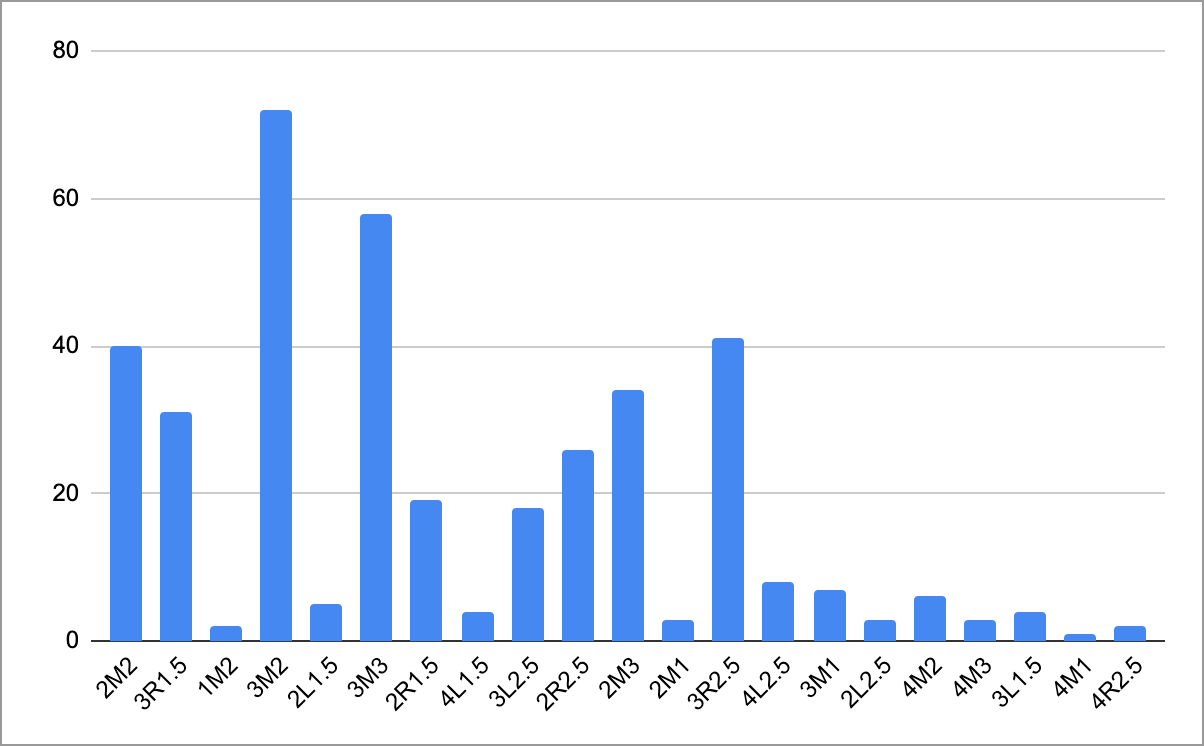
\includegraphics[width=0.9\columnwidth]{pictures/bieu-do-mau-sac-rang.png}
     \caption{Phân bố màu sắc răng hai hàm}
    \label{fig:biểu đồ 3.2}
\end{figure}

\noindent
\textbf{Biểu đồ 3.2.1: Phân bố màu sắc răng hai hàm}\par

\noindent 
\textbf{Nhận xét:}\par
\quad Tỷ lệ màu sắc răng cao nhất ở các đối tượng là màu 3M2, tiếp theo là 3M3 và 3R2.5.\par
\quad Tỷ lệ màu sắc răng thấp nhất là màu 4M1, 4R2.5 và 1M2.


